%File: CAP5512_FinalPaper.tex
%release 2026.0
\documentclass[letterpaper]{article} % DO NOT CHANGE THIS
\usepackage{aaai2026}  % DO NOT CHANGE THIS
\usepackage{times}  % DO NOT CHANGE THIS
\usepackage{helvet}  % DO NOT CHANGE THIS
\usepackage{courier}  % DO NOT CHANGE THIS
\usepackage[hyphens]{url}  % DO NOT CHANGE THIS
\usepackage{graphicx} % DO NOT CHANGE THIS
\urlstyle{rm} % DO NOT CHANGE THIS
\def\UrlFont{\rm}  % DO NOT CHANGE THIS
\usepackage{natbib}  % DO NOT CHANGE THIS AND DO NOT ADD ANY OPTIONS TO IT
\usepackage{caption} % DO NOT CHANGE THIS AND DO NOT ADD ANY OPTIONS TO IT
\frenchspacing  % DO NOT CHANGE THIS
\setlength{\pdfpagewidth}{8.5in}  % DO NOT CHANGE THIS
\setlength{\pdfpageheight}{11in}  % DO NOT CHANGE THIS

\usepackage{algorithm}
\usepackage{algorithmic}
\usepackage{booktabs}
\usepackage{xurl}

\pdfinfo{
/TemplateVersion (2026.1)
}

\setcounter{secnumdepth}{0}

\nocopyright

\title{Hybrid Genetic Algorithm with Simulated Annealing\\for Feature Selection in Network Intrusion Detection}
\author{
    Benedetto Falin,
    Wanis Alshaari,
    Armin Delmo
}
\affiliations{
    Department of Computer Science\\
    University of Central Florida\\
    CAP 5512 --- Spring 2026 --- Dr. Annie Wu
}

\begin{document}

\maketitle

\begin{abstract}
Feature selection in network intrusion detection is a high-dimensional combinatorial optimization problem with $2^{41}$ possible subsets in the NSL-KDD dataset. This paper investigates whether a Hybrid Genetic Algorithm enhanced with Simulated Annealing (GA-SA) produces better feature subsets for binary intrusion detection than a standard Genetic Algorithm alone. Both algorithms are evaluated using a Decision Tree classifier trained on selected feature subsets, with fitness defined as a weighted combination of classification accuracy and feature compactness. Each algorithm is run 10 times across 50 generations and compared across three benchmarks: best fitness convergence, final accuracy, and feature count. Results show that the standard GA achieves higher average fitness and selects fewer features than the hybrid, while both algorithms achieve nearly identical classification accuracy. A Wilcoxon rank-sum test confirms the fitness difference is statistically significant ($p = 0.003$). These findings suggest that the SA component introduces exploration overhead that does not translate into improved generalization and contributes to the understanding of when SA hybridization is and is not justified in population-based feature selection.
\end{abstract}

\section{Introduction}

Modern networks rely heavily on intrusion detection systems (IDS) to identify any malicious traffic. These systems have a large responsibility of monitoring all incoming traffic to stop any malicious activity from traveling through the network. As attack methods become more advanced and networks grow in size, the sheer amount of data that must be processed by IDS keeps increasing. To handle and monitor all of this data, they use many network connection attributes such as protocol type, duration, and error rate to try and gather as much information as possible to detect any incoming attacks. The NSL-KDD dataset is a widely used dataset in network security that reflects this with 41 features describing various attributes of each network connection. However, not all of the included features contribute well towards detection. Some are redundant, some have a high level of noise, and others are irrelevant to finding the malicious traffic. This is a waste in capacity and can cause the model to slow down and perform worse since it wastes time learning from useless data and increases the potential of overfitting. Feature selection becomes an essential preprocessing step for producing intrusion detection models that are both faster and more accurate, which is becoming increasingly important with the rapid growth of networks and the increasing attack threat.

Since feature selection is a combinatorial optimization problem with 41 choices of features, its search space contains $2^{41}$ possible subsets, making any brute-force attempt useless in finding the optimal solution. Genetic Algorithms are a great solution for this and are widely used in machine learning selection tasks similar to this one. The different components of a GA such as selection, crossover, and mutation allow for exploration of the large search space without having to go through every possible solution. However, early convergence is a known issue with GAs where they tend to lose diversity quickly and settle on local optima instead of continuing to explore the search space for better solutions. Simulated Annealing assists in tackling this issue using its temperature-controlled probabilistic acceptance mechanism. It allows the algorithm to escape the local optima by accepting worse solutions early in search of the global optima. As the temperature variable decreases, SA starts being more selective and decreases the amount of worse solutions it allows. Creating a hybrid of a GA with SA combines the GA's global population exploration with SA's local refinement and escape capability.

This study examines whether a hybrid GA-SA can outperform a standard GA for feature selection in the NSL-KDD dataset. Both algorithms are tested and compared under identical conditions to ensure that any performance difference can be attributed to the addition of Simulated Annealing. The performance of each model is measured using classification accuracy, number of selected features, and convergence behavior over generations. Multiple runs are performed to observe consistency across the results. The primary contribution is evidence on whether the hybrid GA truly performs better than the standard GA in feature selection on a real-world network security dataset, and whether the added complexity of Simulated Annealing is justified by improved results.

\section{Related Works}

Prior work in the areas of Genetic Algorithms, Simulated Annealing, and network intrusion detection provides important context for the approach taken in this study. The following works establish the theoretical and applied foundations upon which our hybrid GA-SA feature selection method is built, and highlight the gaps our study seeks to address.

Akula and Kumar tackled the issue of feature selection in intrusion detection using a proposed GA-based feature selection framework evaluated on the NSL-KDD dataset and its 41 features [1]. The main component that differentiated their solution was the use of Stochastic Universal Sampling for selection, combined with Recursive Feature Elimination to remove features irrelevant for detection. They were able to achieve 97.60\% accuracy on the same dataset used in this study. However, their methodology mainly uses multiple external additions on top of the GA to compensate for its limitations in finding the global optima, rather than addressing its search behavior directly. Our approach uses a GA embedded with Simulated Annealing to fight off early convergence at the source.

Bertsimas and Tsitsiklis conducted a deep review of Simulated Annealing and defined it as a method designed to find a global optimum of a cost function when there may be several local maxima within a search space [2]. They found it particularly useful in problems where variables are not independent of each other, such as image classification. This is especially relevant for cybersecurity problems, which tend to have many variables working in tandem, making it hard to find a global optimum in a high-dimensionality search space.

Chiba et al.\ proposed a hybrid optimization framework called GASAA that combines an improved Genetic Algorithm with a Simulated Annealing Algorithm to optimize a Back Propagation Neural Network for anomaly-based network intrusion detection, evaluated on the KDD CUP 99 dataset [3]. In their approach, SA controls the GA's mutation and crossover rates through a temperature variable, starting high to encourage broad exploration and gradually cooling to focus on higher-fitness regions. Their results showed that the GASAA hybrid outperformed both the standalone BPNN and the GA-only version across accuracy, detection rate, and false positive rate metrics. While this work validates the GA-SA hybridization concept in an intrusion detection context, it applies the hybrid to neural network parameter tuning rather than feature selection, and uses the older KDD CUP 99 dataset. Our work builds on this by directing the GA-SA hybrid specifically at the feature selection problem and applying it to the NSL-KDD dataset.

Ghareb et al.\ state that Genetic Algorithms face a known difficulty in that the population always moves toward the best found solution rather than the best possible solution [4]. Their work showed that using an Enhanced Genetic Algorithm with modified crossover and mutation yielded better results in text classification than a typical GA with Naive Bayes. This supports the motivation for hybridization as a means of improving GA search behavior, which is the central approach of our study.

Huang et al.\ proposed SABPIO, an improved binary Pigeon Inspired Optimizer for feature selection on multiple network IDS datasets, which directly integrates Simulated Annealing into the algorithm's search [5]. Their approach was evaluated on NSL-KDD and UNSW-NB15 using Decision Tree and Random Forest classifiers, showing improvement in detection and reduction in selected features compared to the base optimizer. This work is the closest to our proposed approach, as it directly adds SA into a population-based searching algorithm for feature selection in intrusion detection systems. Our study applies this same hybrid concept but uses a GA instead of PIO as the base algorithm.

Jeong et al.\ proposed an optimal feature selection algorithm based solely on Simulated Annealing for detecting six types of Denial of Service attacks within the NSL-KDD dataset [6]. Their SA-based algorithm represents each candidate solution as a binary vector of length 41 and evaluates solutions using a k-means clustering cost function. Results showed that SA-selected subsets achieved competitive accuracy while reducing the average feature count from 41 to approximately 18. While this work demonstrates that SA is a viable standalone mechanism for feature selection on NSL-KDD, it does not explore the benefits of combining SA with a population-based search algorithm. Our work extends this by integrating SA into a Genetic Algorithm framework.

Junghans and Darde demonstrated that combining GA with SA for building optimization produced results closer to the global optimum than a typical GA alone, in some cases improving by as much as 11\% [7]. A similar increase in a cybersecurity setting would be paramount, where false negatives can be detrimental to the safety of individuals' data. This prior success with the GA-SA combination motivated the application of the same hybrid strategy to the feature selection problem in this study.

\section{Experimental Plan}

The goal of our experiment is to determine the differences of using a hybrid GA as opposed to a regular GA for decision tree classification on the NSL-KDD dataset. We would like to see if allowing the GA to explore feature selection is an effective means of achieving high accuracy while also reducing the number of features used. We are using two approaches: a standard GA and a hybrid GA with Simulated Annealing. We believe that using Simulated Annealing alongside a GA will allow individuals of the population to explore different areas within the search space through the temperature factor, generating solutions that may not be at the current apex of the population but can introduce novelty that eventually rises to that level. Once both algorithms have found their most viable solutions at the end of their runs, we compare them against each other to measure statistical significance, accuracy, and feature compactness.

The experiment begins by loading the NSL-KDD dataset using a dedicated dataloader that preprocesses the raw network traffic records into a format suitable for training. The dataset's three categorical features are label encoded, and all labels are converted to a binary classification target where normal traffic is represented as 0 and attack traffic is represented as 1. Min-Max normalization is applied to all feature columns to bring all values into the range $[0, 1]$. The full dataset is preserved and the test set remains completely held out from all selection activity and is only used during fitness evaluation and final reporting.

Both algorithms use a binary individual of length 41, where each bit represents whether a given feature from the NSL-KDD dataset is included or excluded from the selected subset. The fitness of each individual is evaluated using a wrapper approach. To keep evaluation computationally tractable, a 10\% random subsample of the training data is drawn per evaluation using a fixed random state. The selected features are extracted from this subsample using the binary mask, a Decision Tree classifier is trained on that subset, and the classifier is then scored on the full held-out test set. A fitness cache is used to avoid re-evaluating identical chromosomes across the population. The resulting accuracy and the number of selected features are combined into a single fitness score using the weighted formula:

\begin{equation}
    \mathrm{Fitness} = w_1 \cdot \mathrm{Accuracy} + w_2 \cdot \left(1 - \frac{F_{sel}}{F_{total}}\right)
\end{equation}

where $w_1 = 0.8$ and $w_2 = 0.2$. This weighting ensures the algorithm prioritizes predictive performance while still applying pressure to reduce the number of selected features. Both algorithms are run 10 times each with seeds 1 through 10 to account for stochastic variation, and all results are recorded across runs for statistical comparison.

To ensure fair comparison, all core genetic algorithm parameters are standardized and held constant throughout all experimentation. Table~\ref{tab:params} summarizes the shared parameter settings used for both algorithms.

\begin{table}[H]
\centering
\caption{Shared Parameter Settings}
\label{tab:params}
\begin{tabular}{ll}
\toprule
\textbf{Parameter} & \textbf{Value} \\
\midrule
Population Size     & 100 \\
Generations         & 50 \\
Selection           & Tournament ($k = 3$) \\
Crossover           & Single-point, rate 0.8 \\
Mutation            & Bit-flip, rate $1/41$ per bit \\
Elitism             & Top 1 (Hall of Fame) \\
Fitness Weights     & $w_1 = 0.8$, $w_2 = 0.2$ \\
Classifier          & Decision Tree \\
Training Sample     & 10\% subsample (fixed seed) \\
Runs                & 10 \\
\bottomrule
\end{tabular}
\end{table}

The hybrid implementation includes three additional parameters that adjust the Simulated Annealing refinement. Temperature begins at 1.0, allowing nearly all worse solutions to be accepted in early generations. Each generation, the temperature is multiplied by a cooling rate of 0.90, decreasing it by 10\% per generation so that SA becomes increasingly selective over time. Each offspring undergoes 3 iterations of Simulated Annealing per generation. In each iteration, a neighbor is created by flipping a random bit in the chromosome. If the resulting individual has zero features selected, the neighbor is discarded. That neighbor is then evaluated using the Metropolis criterion: if the neighbor's fitness is higher it is always accepted; if it is lower, it is accepted with a probability of $e^{\Delta f / T}$ where $\Delta f$ is the fitness difference and $T$ is the current temperature.

Three benchmarks are used to compare the two algorithms. The first is best fitness convergence over 50 generations, reported as the mean best fitness per generation across all 10 runs. The second is final best accuracy per run, compared via a side-by-side box plot across 10 runs. The third is final best feature count per run, compared via a side-by-side box plot across 10 runs. A Wilcoxon rank-sum test is applied to the final fitness values to assess whether any observed difference is statistically significant.

The proposed hypothesis is that the hybrid GA with SA will achieve better average fitness and classification accuracy across 10 runs due to SA helping offspring escape from local optima that the standard GA would settle in. The hybrid is also expected to select fewer features or an equal number compared to the standard GA.

\section{Results}

Table~\ref{tab:pergen} describes the metrics tracked per generation during each run of both algorithms.

\begin{table}[H]
\centering
\caption{Per-Generation Tracked Metrics}
\label{tab:pergen}
\begin{tabular}{ll}
\toprule
\textbf{Metric} & \textbf{Description} \\
\midrule
Best Fitness       & Highest fitness value in population \\
Average Fitness    & Mean fitness across all individuals \\
Best Accuracy      & Test accuracy of best individual \\
Best Feature Count & Features selected by best individual \\
\bottomrule
\end{tabular}
\end{table}

Table~\ref{tab:perrun} presents the final per-run summary statistics for both algorithms across 10 runs. Each value is the mean and standard deviation of the final best metric at the conclusion of each run.

\begin{table}[H]
\centering
\caption{Per-Run Final Results Across 10 Runs (Mean $\pm$ Std)}
\label{tab:perrun}
\begin{tabular}{lcc}
\toprule
\textbf{Metric} & \textbf{Standard GA} & \textbf{Hybrid GA-SA} \\
\midrule
Best Fitness     & $0.8882 \pm 0.0074$ & $0.8808 \pm 0.0022$ \\
Best Accuracy    & $90.84\%$ & $91.01\%$ \\
Best Feature Count & $7.9$ & $9.7$ \\
\bottomrule
\end{tabular}
\end{table}

% ---------------------------------------------------------------
% CONVERGENCE CURVE FIGURE
% ---------------------------------------------------------------

Figure~\ref{fig:convergence} shows the best fitness convergence curve over 50 generations for both algorithms, where each point on the curve represents the mean best fitness across 10 independent runs. The x-axis is the generation number and the y-axis is the best fitness value in the population.

Both algorithms rise steeply in the first several generations before beginning to slow. Notably, the standard GA (blue) converges to a higher mean best fitness than the Hybrid GA-SA (orange) throughout all 50 generations, reaching a mean of 0.8882 compared to the hybrid's 0.8808 by the final generation. This result is counterintuitive relative to the hypothesis and indicates that the SA component does not improve the best individual found per generation. Instead, the SA refinement step appears to disturb well-performing individuals by accepting worse solutions, which limits the population's ability to concentrate around the highest-fitness region of the search space. 

A Wilcoxon rank-sum test on the final best fitness values across 10 runs yielded $p = 0.003$, confirming that this advantage for the standard GA is statistically significant and not the result of random variation.
\\
\begin{figure}[t]
    \centering
    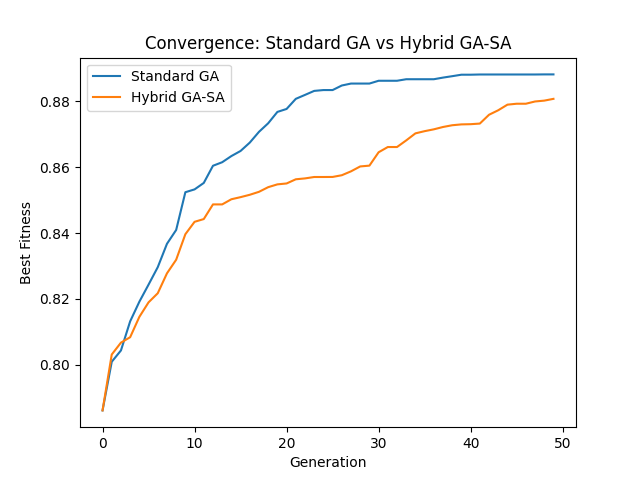
\includegraphics[width=\columnwidth]{images/convergence_GAs.png}
    \caption{Best fitness convergence over 50 generations for the standard GA (blue) and Hybrid GA-SA (orange), averaged across 10 runs.}
    \label{fig:convergence}
\end{figure}

% ---------------------------------------------------------------
% RANK-SUM TEST TABLE
% ---------------------------------------------------------------

Table~\ref{tab:wilcoxon} presents the results of a Wilcoxon rank-sum test, also known as the Mann-Whitney U test, applied to the final best fitness values collected across 10 runs for each algorithm. The test component column describes each element of the statistical test and the value column provides the corresponding result. The test was chosen because it makes no assumption about the underlying distribution of fitness values, which is appropriate given the small sample size of 10 runs per algorithm. The resulting $p$-value of 0.003184 falls well below the significance threshold of $\alpha = 0.05$, indicating that the difference in final fitness between the standard GA and the Hybrid GA-SA is statistically significant and is not attributable to random variation across runs. The test favors the standard GA, confirming that its higher average fitness of 0.8882 compared to the hybrid's 0.8808 represents a genuine performance difference under these experimental conditions.

\begin{table}[t]
\centering
\caption{Statistical Significance Test on Final Fitness}
\label{tab:wilcoxon}
\begin{tabular}{ll}
\toprule
\textbf{Component} & \textbf{Value} \\
\midrule
Test Used          & Wilcoxon Rank-Sum\\
Compared Metric    & Final best fitness \\
Runs per Algorithm & 10 \\
$p$-value          & 0.003184 \\
Significance Level & $\alpha = 0.05$ \\
Conclusion         & Statistically significant difference \\
Favored Algorithm  & Standard GA \\
\bottomrule
\end{tabular}
\end{table}

Taken together, the results tell a coherent story. The standard GA achieves higher fitness and selects fewer features while producing a classifier of nearly identical accuracy to the hybrid. The SA component's exploration overhead does not produce a better solution in this experimental configuration and comes at the cost of selecting more features and lower measured fitness. The Wilcoxon rank-sum test confirms that the standard GA's fitness advantage is statistically significant at $p = 0.003$.

\section{Conclusions}

This study examined whether a Hybrid Genetic Algorithm enhanced with Simulated Annealing outperforms a standard GA for feature selection in the NSL-KDD network intrusion detection dataset. The motivation was that standard GAs are known to converge prematurely on local optima in high-dimensional combinatorial spaces, and SA's temperature-controlled acceptance mechanism was hypothesized to address this limitation by enabling the population to explore more of the search space and find better feature subsets.

Both algorithms were evaluated over 10 independent runs of 50 generations each using a Decision Tree classifier. Fitness was defined as a weighted combination of classification accuracy on the held-out test set and feature compactness, with weights of 0.8 and 0.2 respectively. A 10\% subsample of the training data was used per fitness evaluation to keep computation tractable, and a fitness cache prevented redundant evaluations of identical chromosomes.

Contrary to the hypothesis, the standard GA outperformed the hybrid in average best fitness (0.8882 vs 0.8808), with the difference confirmed as statistically significant by a Wilcoxon rank-sum test ($p = 0.003$). Both algorithms achieved nearly identical test set accuracy of approximately 90.84\% and 91.01\% respectively, a difference of 0.17 percentage points. The standard GA also selected fewer features on average, 7.9 compared to the hybrid's 9.7, indicating that the SA component produced less compact feature subsets rather than leaner ones as hypothesized.

These findings suggest that in this experimental configuration, the SA refinement step disturbs well-performing individuals by accepting worse solutions, which limits the population's convergence to the highest-fitness region of the search space. The standard GA's faster convergence acts as an implicit regularizer that produces compact and competitive feature subsets without the overhead of local perturbation.

The contribution of this work is a direct empirical comparison of standard and hybrid GA feature selection under controlled conditions on a real-world network security dataset, with statistical validation via the Wilcoxon rank-sum test. The results indicate that the justification for SA hybridization in feature selection depends on careful tuning of the SA parameters and fitness weighting. Future work should explore adjusted cooling schedules, stronger feature compactness penalties, and a larger number of runs to determine under what conditions the GA-SA hybrid provides a meaningful advantage over a standard GA.

\newpage

\section{References}

\begin{enumerate}

    \item \label{akula2025} Akula, R., \& Kumar, G. S. N. (2025). Optimizing feature selection in intrusion detection systems using a genetic algorithm with stochastic universal sampling. \textit{International Journal of Advanced Computer Science and Applications, 16}(1). \url{https://thesai.org/Downloads/Volume16No1/Paper_102-Optimizing_Feature_Selection_in_Intrusion_Detection_Systems.pdf}

    \item \label{bertsimas1993} Bertsimas, D., \& Tsitsiklis, J. (1993). Simulated annealing. \textit{Statistical Science, 8}(1), 10--15. \url{https://doi.org/10.1214/ss/1177011077}

    \item \label{chiba2019} Chiba, Z., Abghour, N., Moussaid, K., El Omri, A., \& Rida, M. (2019). A hybrid optimization framework based on genetic algorithm and simulated annealing algorithm to enhance performance of anomaly network intrusion detection system based on BP neural network. \textit{IEEE Xplore}. \url{https://ieeexplore.ieee.org/document/8618804/}

    \item \label{ghareb2016} Ghareb, A. S., Bakar, A. A., \& Hamdan, A. R. (2016). Hybrid feature selection based on enhanced genetic algorithm for text categorization. \textit{Expert Systems with Applications, 49}, 31--47. \url{https://doi.org/10.1016/j.eswa.2015.12.004}

    \item \label{huang2024} Huang, W., Tian, H., Wang, S., Zhang, C., \& Zhang, X. (2024). Integration of simulated annealing into pigeon inspired optimizer algorithm for feature selection in network intrusion detection systems. \textit{PeerJ Computer Science, 10}, e2176. \url{https://doi.org/10.7717/peerj-cs.2176}

    \item \label{jeong2016} Jeong, I.-S., Kim, H.-K., Kim, T.-H., Lee, D. H., Kim, K. J., \& Kang, S.-H. (2016). A feature selection approach based on simulated annealing for detecting various denial of service attacks. \textit{Journal of Convergence Security, 1}, 1--18. \url{https://www.semanticscholar.org/paper/A-Feature-Selection-Approach-Based-on-Simulated-for-Jeong-Kim/3282c78abb7840a2fb16e3261247640944f3f816}

    \item \label{junghans2015} Junghans, L., \& Darde, N. (2015). Hybrid single objective genetic algorithm coupled with the simulated annealing optimization method for building optimization. \textit{Energy and Buildings, 86}, 651--662. \url{https://doi.org/10.1016/j.enbuild.2014.10.039}

\end{enumerate}

\end{document}